\documentclass{article}
\usepackage{graphicx}
\usepackage[margin=1.5cm]{geometry}
\usepackage{amsmath}

\begin{document}

\title{Thursday Reading Assessment: Chapter 2-8, 2-10 through 2-12}
\author{Prof. Jordan C. Hanson}

\maketitle

\section{Binary, Hexadecimal, BCD, and Gray Codes}

\begin{enumerate}
\item Let $x_1 = 10110$.  Show that taking the 2's complement of $x_1$ \textit{twice} returns $x_1$. \\ \vspace{0.15cm}
\item Show that the range of 4-bit signed binary numbers in 2's complement form is $[-8,7]$, assuming one sign bit. \\ \vspace{0.25cm}
\item Let $x_1 = F7_{16}$, and $x_2 = 9D_{16}$.
\begin{enumerate}
\item What is $x_1$ in binary? \\ \vspace{0.25cm}
\item What is $x_2$ in decimal? \\ \vspace{0.25cm}
\end{enumerate}
\item Imagine a stream of binary digits coming through a serial line.  They are: $1001 ... 0001 ... 0001$.  If we know the bitstream is in binary coded decimal (BCD), what is the code being sent? \\ \vspace{0.25cm}
\item What property of the four-bit gray code in Fig. \ref{fig:gray} distinguishes it from straight binary counting?
\begin{figure}[hb]
\centering
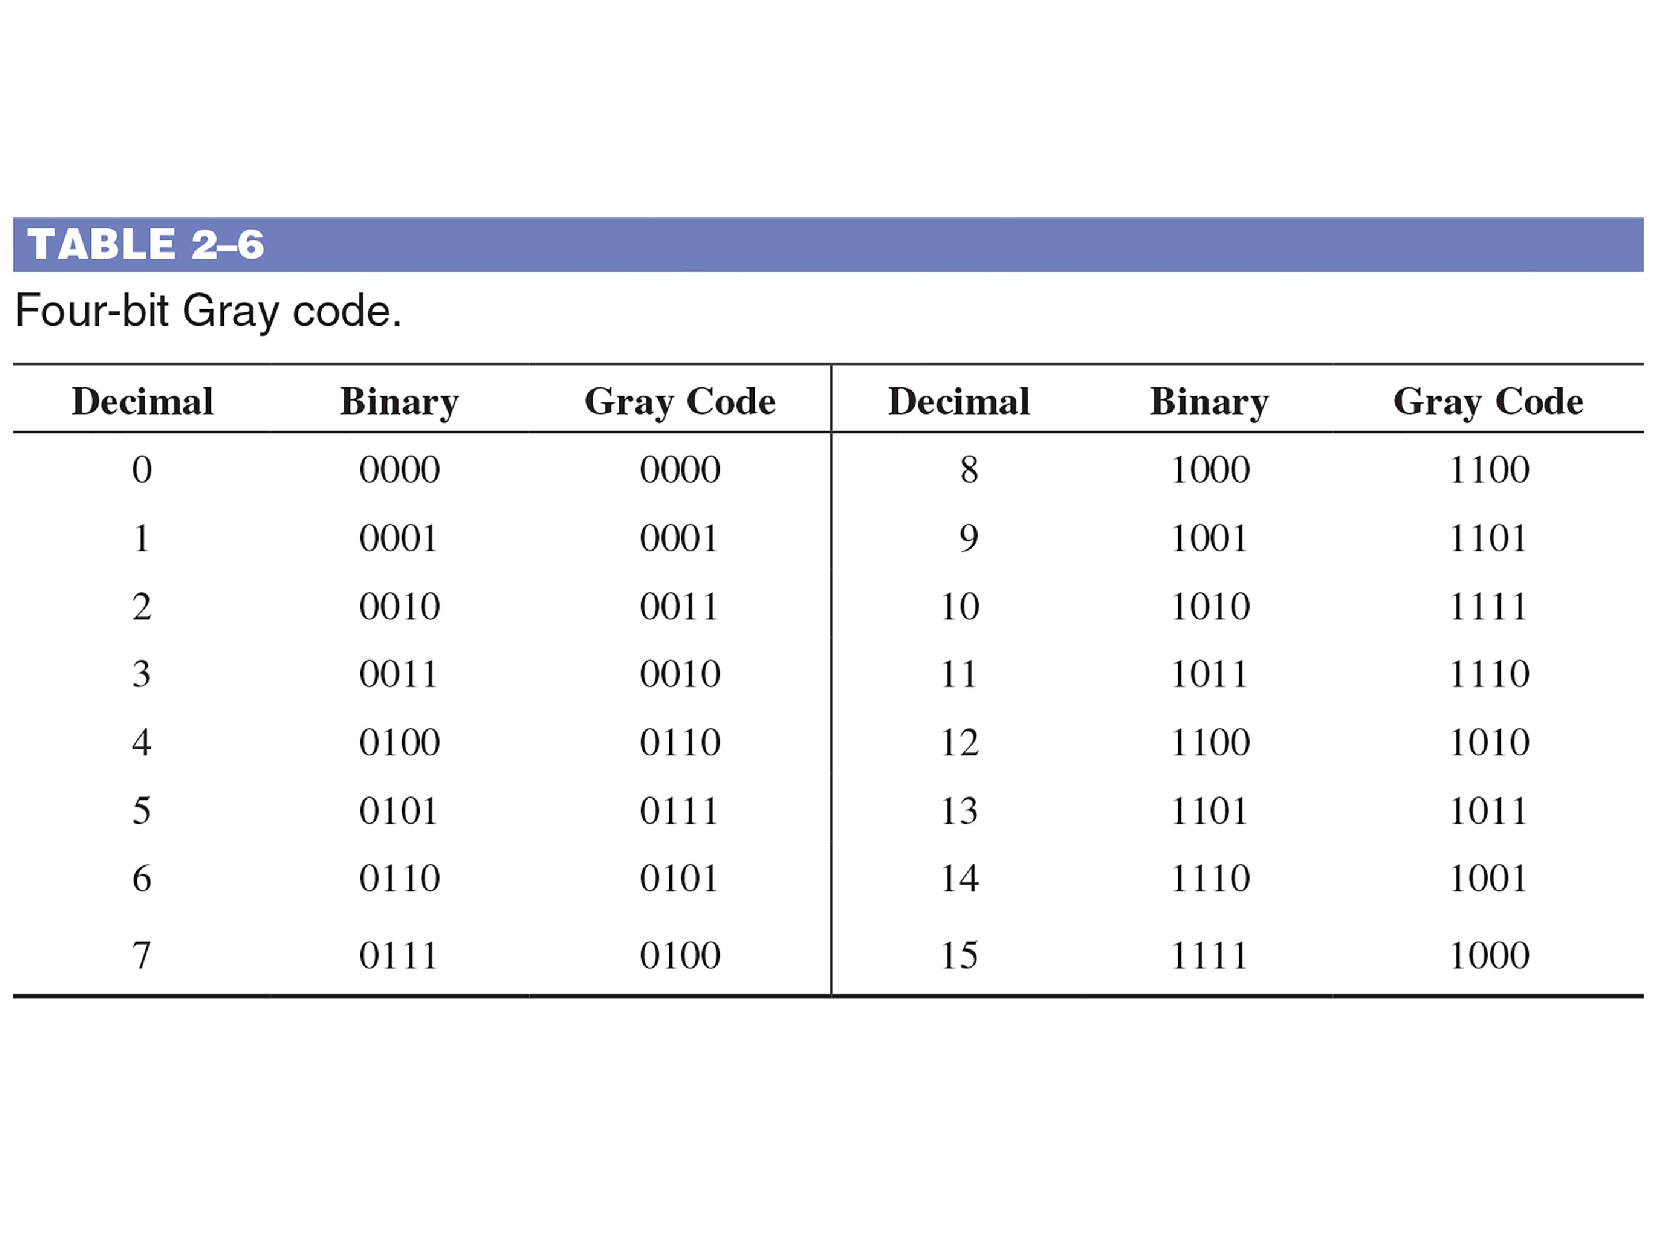
\includegraphics[width=0.5\textwidth,trim=0cm 3cm 0cm 0cm,clip=true]{figures/gray.pdf}
\caption{\label{fig:gray} A four-bit binary gray code.}
\end{figure}
\item Convert 1010 (gray code) to binary, showing how the process works. \\ \vspace{0.5cm}
\item Circle all the following 4-bit BCD code word sequences below that have a \textit{single-bit} error, assuming \textit{even} parity:
\begin{itemize}
\item 1 0011 0010
\item 0 1110 1010
\item 1 0111 1110 1000 1010
\end{itemize}
\end{enumerate}

\end{document}
